%%% ===============================================================================
\chapter{Introduction}\label{sec:introduction}
%%% ===============================================================================

\emph{Purpose and scope of your entire report}.
The purpose of your entire report is to make a \emph{scientific argument using the scientific method}. \gls{rdbms}
A scientific argument always has the following steps that all must come in this order.
%
\begin{itemize}
  \item[SM1] \emph{Explicate the assumptions and state of the art} on which you are going to conduct your research to investigate your research problem/test the hypothesis.
  \item[SM2] Clearly and precisely \emph{formulate a research problem or hypothesis}.
  \item[SM3] \emph{Describe the (research) method} that you followed to investigate the problem / to test the hypothesis in a way that \emph{allows someone else to reproduce your steps}.
        The method must includes steps and criteria for evaluating whether you answered your question successfully or not.
  \item[SM4] \emph{Provide execution details} on how you followed the method in the given, specific situation.
  \item[SM5] \emph{Report your results} by describing and summarizing your measurements.
        You must not interpret your results.
  \item[SM6] \emph{Now interpret your results} by contextualizing the measurements and drawing conclusion that lead to answering your research problem or defining further follow-up research problems.
\end{itemize}
%
This template will mark various parts of the structure with SM1-SM6 to recall to you which step of a scientific argument is used and where.

\emph{Purpose and scope of \zcref{sec:introduction}}.
The introduction chapter is a summary of your work and your scientific argument that must be understandable to anyone in your scientific field, e.g., anyone in Data Science.
A reader must be able to comprehend the problem, method, relevant execution details, results, and their interpretation by reading the introduction and the introduction alone.
Section~\ref{sec:introduction:topic} introduces the general topic of your research.
Section~\ref{sec:introduction:state-of-art} discusses the state of the art and identifies a research.
Section~\ref{sec:introduction:research-question} then states the research problem to investigate.
Section~\ref{sec:problem-exposition:research-method} explains the research method that was followed, possibly with execution details.
Section~\ref{sec:introduction:results} then presents the results and their interpretation.
A reader should need to read further only if they are not convinced or need more details to reproduce your study.
The individual chapters and sections provide the details for each of the steps in your scientific argument.

You usually write the introduction chapter \emph{after} you wrote all other chapters, but you should keep on making notes for each of the sections as you write the later chapters.
.

\emph{Purpose and scope of the introduction paragraph to a chapter}.
The paragraph you are reading above is a typical introductory paragraph to a chapter.
It is a high-level summary of the chapters' topic (SM1 and SM2).
It gives the reader some guidance by breaking down the chapter topic into subtopics that are named (SM3) in the right order with forward references to the corresponding sections (SM4).
It may close with announcing the result you obtain (SM6) but this is usually not done in the opening paragraph of the introduction.

\emph{Two kinds of readers}.
Write your report so that it can be read from beginning to end: introduce every concept before you use it.
Backward references are fine; forward references in the running text should be rare.
At the same time, guide the reader who opens your report somewhere and has ten minutes:
each chapter starts with an introductory paragraph as described above, which outlines the coming sections and links back to what the chapter builds on and forward to where its results are used.
The book \enquote{Student Thesis Projects}~\cite{Lichter2026} (open access) explains in detail how to organize, conduct, write, and present a thesis.
Before you hand in, work through the checklist in \href{https://github.com/latextemplates/scientific-thesis-template/blob/main/docs/thesis-checklist.md}{\texttt{docs/thesis-checklist.md}} and remove all these hints.

% ---------------------------------------------------------------------------------
\section{Context and Topic (SM1)}\label{sec:introduction:topic}
% ---------------------------------------------------------------------------------

\emph{Purpose and scope}.
You begin with providing the general scientific audience an introduction into the specific topic of your work.
The aim of this section is to first introduce the \emph{general subject of study} (``Giraffes are well-known animals and everyone's favorite''), the \emph{specific topic of societal or scientific interest} to investigate (``Giraffes have blue tongues'') and the \emph{objective of society/science towards} this topic (``it is unknown at the moment how the blue color tone evolved'').
It must be understandable by the general scientific public.
Every \emph{term} with a specific meaning must be highlighted and introduced in precise language/concepts that only builds on a general scientific background.

At the end of this section, you have explained and established a general goal that society/science universally agrees to be worth achieving (``knowing how everyone's favorite animal evolved the colour of their tongue'').

% ---------------------------------------------------------------------------------
\section{State of the Art (SM1)}\label{sec:introduction:state-of-art}
% ---------------------------------------------------------------------------------

\emph{Purpose and scope}.
You provide a more in-depth introduction into the research topic by contrasting the current state of the art in society/science in relation to the research topic you introduced in \zcref{sec:introduction:topic}.
This introduction has to

\begin{itemize}
  \item present established facts, methods, and results that provide a deeper understanding of the research topic (``prior work on giraffe genomes, relevance of giraffes for societal well-being, giraffes being a model-animal for various other studies, etc.'')
  \item discuss in which ways prior and recent ideas still fall short of reaching the general goal you explained in \zcref{sec:introduction:topic} (``prior work only sequenced the genome of one giraffe and did not consider genes of ancient ancestors'')
\end{itemize}

You have to provide citations/literature references for each of the statements and claims you are making.
This section is usually a summary of the related work discussion in \zcref{sec:background}.

At the end of this section, you have established a \emph{knowledge gap} between the state of the art and the general objective you developed in \zcref{sec:introduction:topic}.
\emph{Stating a (knowledge) gap between a status quo and a desired situation is the \emph{first step} of a writing scientific argument.}

% ---------------------------------------------------------------------------------
\section{Research Question (SM2)}\label{sec:introduction:research-question}
% ---------------------------------------------------------------------------------

\emph{Purpose and scope}.
In this section you state in which way you will address the knowledge gap you identified at the end of \zcref{sec:introduction:state-of-art}.
You usually cannot address and resolve the entire knowledge gap in your work.
The purpose of this section is to detail the specific part of the knowledge that you will address.
You thereby make all the assumptions explicit that underlie your work (``in this report we focus on genomes of female giraffes who lived in the years 1950-2000 in South Africa'').

Your general research question states
\begin{itemize}
  \item The starting point/assumptions you are making from which your research starts (``for the given 13 genomes of female giraffes...''), and
  \item the final objective/solution you want to reach (``...identify the genes involved in color expression of giraffe tongues...'')
  \item and the evaluation criteria that will determine whether you are successful (``...that are present in at least 75\% of the studied giraffes'')
\end{itemize}

You will usually break your general research question down into sub-research questions.
You may do this here.
The sub-research questions have to form a chain that take you in smaller steps from the starting point/assumptions of your general research question to your final objective and evaluation.

% ---------------------------------------------------------------------------------
\section{Method or Approach (SM3, SM4)}\label{sec:introduction:method}
% ---------------------------------------------------------------------------------

\emph{Purpose and scope}.
In this section you outline the method that you applied to answer the research questions, or the new technical approach that you developed to answer it.
It is a summary of the steps that someone else has to take in order to reproduce your steps.
Mention here the data sets you had to obtain/gather/analyze, interviews with stakeholders you had to make to further develop the research questions, technical artifacts (programs, algorithms, models) you could apply or that you had to develop (and how they work).

The section is most readable if you give each of the steps in your method its own paragraph.
In each paragraph you first briefly explain the concept of the step in your method (SM3, ``we explored the data through visual analytics'') and then provide details in execution (SM4, ``we used tool X, we developed dashboard Y'') include a forward reference to the respective chapter that provides more details.

% ---------------------------------------------------------------------------------
\section{Findings (SM5, SM6)}\label{sec:introduction:results}
% ---------------------------------------------------------------------------------

\emph{Purpose and scope}.
You close the introduction by stating the evaluation setup you designed to evaluate the success of your study regarding the research objective, which comes in two steps.
It is most likely a summary of your evaluation in \zcref{sec:evaluation}.

\section*{Results (SM5)}

You state the evaluation method that is in line with your research question from \zcref{sec:introduction:research-question} and summarize the measurements you obtained but you do not interpret them, i.e., you only report the numbers but you do not include judging statements.

\section*{Interpretation (SM6)}

You summarize your interpretation of the results and draw conclusions.
State whether and to which degree the research question from \zcref{sec:introduction:research-question} has been answered successfully or not.

Finally state briefly how much closer society and science have come in answering the general objective you outlined in \zcref{sec:introduction:topic}.

%%% ===============================================================================
\section{Background (SM1)}\label{sec:background}
%%% ===============================================================================

\emph{Purpose and scope}.
The background chapter has multiple roles.
\begin{itemize}

  \item \emph{Preliminaries.}
        It has to provide all (and exactly the) information that is necessary to understand the methodological and technical parts of your work in the specific area of study.
        Assume as starting point another student in your degree who did not study the specific subject you are studying but has the task to understand your work.
        Which concepts, terms, definitions, etc. does the student have to know?
        Which formulas, symbols, etc. are standard in this topic?
        Only introduce definitions if you actually need them in any of the subsequent chapters.

  \item \emph{Related Work.}
        It has to provide a comprehensive discussion of all prior work in the area on this subject.
        Your discussion has to summarize these prior works and has to explain in which way the research question you are solving (\zcref{sec:introduction:research-question}) has not bee solved yet because prior work had more limiting assumptions, addressed a different angle, their results are not complete etc. Depending on the subject you are studying, the related work part can be larger and warrant an entire chapter on its own, or be fully concluded within \zcref{sec:introduction:state-of-art}.

        You can close the related work discussion by clarifying the positioning and formulation of your research question (SM2) in relation to all the prior work, making more explicit whether you address an existing research question under different premises or whether you work on a modified or completely new research question.
\end{itemize}

%%% ===============================================================================
\section{Problem Exposition (optional)}\label{sec:problem-exposition}
%%% ===============================================================================

\emph{Purpose and scope}.
Introduce the problem context in more detail if \zcref{sec:introduction:topic} does not provide all necessary information about the problem to follow the rest of the report.
This can include further details on the data you studied, context assumptions and requirements, etc.

If you have to expose the problem in more detail here, then this chapter should also provide a more detailed explanation of research question and the method you are applying, i.e., you can now provide more concrete sub-problems compared to \zcref{sec:introduction:research-question} more details for the method \zcref{sec:introduction:method} because you now have explained the problem much better.
A typical structure can be.

% ---------------------------------------------------------------------------------
\section{Context/Business Understanding (SM1)}\label{sec:problem-exposition:context-understanding}
% ---------------------------------------------------------------------------------

provide details

% ---------------------------------------------------------------------------------
\section{Data Understanding (SM1)}\label{sec:problem-exposition:data-understanding}
% ---------------------------------------------------------------------------------

provide details

% ---------------------------------------------------------------------------------
\section{Detailed Research Questions (SM2)}\label{sec:problem-exposition:research-problems}
% ---------------------------------------------------------------------------------

provide details based on \zcref{sec:problem-exposition:context-understanding} and \ref{sec:problem-exposition:data-understanding}

% ---------------------------------------------------------------------------------
\section{Detailed Method (SM3)}\label{sec:problem-exposition:research-method}
% ---------------------------------------------------------------------------------

provide details based on \zcref{sec:problem-exposition:context-understanding} and \ref{sec:problem-exposition:data-understanding}

%%% ===============================================================================
\section{First Real Chapter addressing first Research Problem}\label{sec:problem1}
%%% ===============================================================================

\emph{Purpose and scope}.
After you stated research context (SM1), research problem (SM2), and research method (SM3) in \zcref{sec:introduction} and possibly \zcref{sec:problem-exposition}, the remainder of your entire report addresses execution (SM4), results (SM5), and interpretation (SM6).
You usually do this by addressing various sub-problems again through scientific arguments following the 6 steps SM1-SM6.

Have a short chapter introduction that recalls and explains the first research problem of your thesis.
The problem has to show up in the introduction in \zcref{sec:introduction:research-question} or in \zcref{sec:problem-exposition:research-problems} already.
This provides the background (SM1) for this chapter while the first research problem of the thesis becomes the research question/hypothesis (SM2) for this chapter.

Next, explain in the chapter intro how you solve the research problem in this chapter by breaking it down in further sub-problems.
By this, you outline the method (SM3) through which you are going to solve the problem of this chapter.
This is necessary to give the reader guidance of what's to come in this chapter and how it fits into the thesis as a whole.
Explain that you will address the first sub-problem in \zcref{sec:problem1:subproblem1} and the second sub-problem in \zcref{sec:problem1:subproblem2}, etc. The sections then provide the details for execution and results.

% ---------------------------------------------------------------------------------
\section{First Sub-Problem}\label{sec:problem1:subproblem1}
% ---------------------------------------------------------------------------------

\emph{The first paragraph describes the first sub-problem and develops the requirements a solution has to satisfy (SM2 for this section).}
The requirements have to be based on the knowledge and reasoning developing in the preceding chapters and sections.
Try to use an example to illustrate the problem and the desired properties of the solution.
Check that every term/concept you use here has already been defined already in a previous section.
If you cannot describe your problem without defining new terms, you may have to add another section before this one that develops the terms and concepts you need to explain the problem.

\emph{The second paragraph describes the method/approach how you address the problem (SM3 for this section).}
Describe the method in a level of detail that allows another student to reproduce your steps.
Make use of appendices % (see \zcref{sec:appendix1})
if certain details take too much space.

\emph{The third, fourth, and following paragraph provides details on applying the method or developing a new approach, i.e., execution (SM4) and may explain results (SM5)}, i.e. details on the steps needed to reproduce the results.

Results (SM5) can come in many forms, e.g., conceptual diagrams, algorithms, tables, charts, a list of articles from a literature research etc. You must reference them (``\zcref{fig:my_label} shows.
..'') and describe the results in text.
If you use diagrams, tables, or charts, you cannot expect the reader to know what to you expect them to see in a diagram, table or chart.
Describe to them how to read these, explain the meaning of particular elements, point out special observations.
Describe the results, but do not interpret them.
Make use of appendices if certain details take too much space.

\begin{figure}
  \centering
  %%%\includegraphics{/path/to/figure.pdf}
  \caption{A scientific figure that has to be explained in the text}
  \label{fig:my_label}
\end{figure}

\emph{After describing the results, you may interpret them (SM6).}
Here you can infer what a particular observation means (for you), how it can be applied, or what others can do with it.
Do not interpret your results before you have described all of them.
This is a common mistake done by most beginner writers.
You want to quickly get to the point, which is the final finding or interpretation.
But you forget that your reader does not understand yet what you are interpreting - they do not know yet what you do know.
Interpret the results only after describing all of them.
The interpretation must be based on the written description only.
Then you can be sure that your readers can follow your interpretation and reach the same conclusions as you have.

Ideally, your interpretation leads to the next sub-problem in \zcref{sec:problem1:subproblem2}.

% ---------------------------------------------------------------------------------
\section{Second Sub-Problem}\label{sec:problem1:subproblem2}
% ---------------------------------------------------------------------------------

You now build on the solution to the first sub-problem of \zcref{sec:problem1:subproblem1} (SM1) and recall second sub-problem (SM2, you detailed in the introduction of this chapter) and follow the same pattern as before (SM3-SM6).

Note that not all sections may not include all parts SM1-SM6 in all detail.
Some sections need not restate the background (SM1) or the research problem (SM2) if a previous section already defined them.
Sometimes, a section is only dedicated to describing the method (SM3) and execution (SM4) and does not contain any results or interpretations.
Sometimes results (SM5) and interpretations (SM6) only come in the evaluation chapter.

What is important for you when you are writing a scientific argument is not to slavishly have SM1-SM6 in each section explicitly, but that you are always fully aware of the following:
%
\begin{itemize}
  \item Which step of a scientific argument am I currently writing (SM1, SM2, ..., SM6)?
  \item Does the step that I am writing come in the right order, i.e., if you are writing about execution (SM4, e.g., details of building a model), is there a preceding paragraph or section that describes the method (SM3) and is that one preceded by a clear statement of the (sub-)problem addressed (SM2)?
  \item Are you really \emph{not} writing interpretation SM6 before SM5, SM4, or SM3?
  \item Is it clear to the reader which part of the scientific argument you are currently making?
\end{itemize}

%%% ===============================================================================
\section{Second Real Chapter}\label{sec:sub-problem2}
%%% ===============================================================================

Have a short chapter introduction that recalls what you already achieved in \zcref{sec:problem1} and explain the second research problem of your thesis.
The problem has to show up in the introduction in \zcref{sec:introduction:research-question} or in \zcref{sec:problem-exposition:research-problems} already.
etc.

%%% ===============================================================================
\section{Evaluation}\label{sec:evaluation}
%%% ===============================================================================

\emph{Purpose and scope}.
The evaluation chapter should be the most formal and rigorously structured chapter of your thesis as the validity of your evaluation argument depends on it.

% ---------------------------------------------------------------------------------
\section{Objective (SM2)}\label{sec:evaluation:objective}
% ---------------------------------------------------------------------------------

State what you want to evaluate and what you want to measure.

% ---------------------------------------------------------------------------------
\section{Setup (SM3)}\label{sec:evaluation:setup}
% ---------------------------------------------------------------------------------

State which data, participants, tools, etc. you chose and why.
State how you measure outcomes and how you compare them to baselines, reference groups, etc.

% ---------------------------------------------------------------------------------
\section{Execution (SM4)}\label{sec:evaluation:execution}
% ---------------------------------------------------------------------------------

Provide all details on the execution that are necessary to allows another person to reproduce your results at a later point.

% ---------------------------------------------------------------------------------
\section{Results (SM5)}\label{sec:evaluation:results}
% ---------------------------------------------------------------------------------

You only report the measurements.
You must present and reference them (``\zcref{fig:my_label2} shows.
..'') and describe the results in text.
If you use diagrams, tables, or charts, you cannot expect the reader to know what to you expect them to see in a diagram, table or chart.
Describe to them how to read these, explain the meaning of particular elements, point out special observations.
Describe the results, but do not interpret them.
Make use of appendices if certain details take too much space.

\begin{figure}
  \centering
  %%%\includegraphics{/path/to/figure.pdf}
  \caption{Another scientific figure that has to be explained in the text}
  \label{fig:my_label2}
\end{figure}

% ---------------------------------------------------------------------------------
\section{Discussion (SM6)}\label{sec:evaluation:discussion}
% ---------------------------------------------------------------------------------

Interpret the results only after describing all of them.
The interpretation must be based on the written description in \zcref{sec:evaluation:results} only.
Then you can be sure that your readers can follow your interpretation and reach the same conclusions as you have.


%%% ===============================================================================
\chapter{Conclusion and Outlook}\label{sec:conclusion}
%%% ===============================================================================

Your conclusions are not just a factual summary of your work, but they position, interpret, and defend your findings against the state of the art that you discussed in \zcref{sec:introduction:state-of-art}.
You specifically outline which concrete findings or methodological contributions advance our knowledge towards the general objective you introduced in \zcref{sec:introduction:topic}.
Objectively discuss which parts you solved and in which parts you failed.

You should explicitly discuss limitations and shortcomings of your work and detail what kind of future studies are needed to overcome these limitations.
Be specific in the sense that your arguments for future work should be based on concrete findings and insights you obtained in your report.


\chapter{LaTeX Hints}
\label{sec:latexhints}

% Required for proper example rendering in the compiled PDF
\newcount\LTGbeginlineexample
\newcount\LTGendlineexample
\newenvironment{ltgexample}%
{\LTGbeginlineexample=\numexpr\inputlineno+1\relax}%
{\LTGendlineexample=\numexpr\inputlineno-1\relax%
  \tcbinputlisting{%
    listing only,
    listing file=\currfilepath,
    colback=green!5!white,
    colframe=green!25,
    coltitle=black!90,
    coltext=black!90,
    left=8mm,
    title=Corresponding \LaTeX{} code of \texttt{\currfilepath},
    listing options={
        frame=none,
        language={[LaTeX]TeX},
        escapeinside={},
        firstline=\the\LTGbeginlineexample,
        lastline=\the\LTGendlineexample,
        firstnumber=\the\LTGbeginlineexample,
        basewidth=.5em,
        aboveskip=0mm,
        belowskip=0mm,
        numbers=left,
        xleftmargin=0mm,
        numberstyle=\tiny,
        numbersep=8pt%
      }
  }
}%

This chapter contains hints on writing LaTeX.
It focuses on minimal examples, which can be directly adapted to the content

\section{Handling of paragraphs}

\begin{ltgexample}
One sentence per line.
This rule is important for the usage of version control systems.
A new line is generated with a blank line.
As you would do in Word:
New paragraphs are generated by pressing enter.
In LaTeX, this does not lead to a new paragraph as LaTeX joins subsequent lines.
To start a new paragraph, press enter twice.
This leads to an empty line.
In word, there is the functionality to press shift and enter.
This leads to a hard line break.
The text starts at the beginning of a new line.
In LaTeX, you can do that by using two backslashes (\textbackslash\textbackslash).
\\
This is rarely used.

Please do \textit{not} use two backslashes for new paragraphs.
For instance, this sentence belongs to the same paragraph, whereas the last one started a new one.
A long motivation for that is provided at \url{http://loopspace.mathforge.org/HowDidIDoThat/TeX/VCS/#section.3}.
\end{ltgexample}

\section{Notes separated from the text}

The package mindflow enables writing down notes and annotations in a way so that they are separated from the main text.

\begin{ltgexample}
\begin{mindflow}
This is a small note.
\end{mindflow}
\end{ltgexample}

\section{Handling TODOs}

\begin{ltgexample}
\textmarker{Marked text.}
\end{ltgexample}

With \verb1\textmarker1, only the text color is changed, since this also works well for individual words.

\begin{ltgexample}
\textcomment{Marked text.}{A comment on it.}
\end{ltgexample}

\begin{ltgexample}
\hl{Highlighted in yellow.}
Provided indirectly by pdfcomment.sty (soulpos).
\end{ltgexample}

\begin{ltgexample}
\modified{Manual marking for text that has been changed since the last version.}
\end{ltgexample}

\begin{ltgexample}
This is some text.
\change{FL1: text adjusted}{Changed text}.
\end{ltgexample}

\begin{ltgexample}
Here is a comment\sidecomment{Comment}.
\end{ltgexample}

\begin{ltgexample}
\todo{A lot of text still needs to be produced here}
\end{ltgexample}

\section{Hyphenation}

\LaTeX{} automatically hyphenates words.
When using \href{https://ctan.org/pkg/microtype}{microtype}, there should be fewer hyphenations than in other settings.
You might still need to tweak the hyphenation.
Here are some hints:

\begin{ltgexample}
In case you write \enquote{application-specific}, then the word will only be hyphenated at the dash.
You can also write \verb1applica\allowbreak{}tion-specific1 (result: applica\allowbreak{}tion-specific), but this is much more effort.

You can now write words containing hyphens which are hyphenated at other places in the word.
For instance, \verb1application"=specific1 gets application"=specific.
This is enabled by an additional configuration of the babel package.
\end{ltgexample}

\section{Typesetting Units}

\begin{ltgexample}
Numbers can be written plain text (such as 100), by using the \href{https://ctan.org/pkg/siunitx}{siunitx} package as follows:
\SI{100}{\km\per\hour},
or by using plain \LaTeX{} (and math mode):
$100 \frac{\mathit{km}}{h}$.
\end{ltgexample}

\begin{ltgexample}
\SI{5}{\percent} of \SI{10}{kg}
\end{ltgexample}

\begin{ltgexample}
Numbers are automatically grouped: \num{123456}.
\end{ltgexample}

\section{Surrounding Text by Quotes}

\begin{ltgexample}
Please use the \enquote{enquote command} to quote something.
Quoting with "`quote"' or ``quote'' also works.

\end{ltgexample}

\section{Zref-clever examples}
\label{sec:ex:cref}

zref-clever demonstration: Zcref (short for zcref[S]) at beginning of sentence, zcref in all other cases.

\begin{figure}
  \centering
  \includegraphics[width=.75\linewidth]{example-image-a}
  \caption{Example figure for zcref demo}
  \label{fig:ex:cref}
\end{figure}

\begin{table}
  \centering
  \begin{tabular}{ll}
    \toprule
    Heading1 & Heading2 \\
    \midrule
    One      & Two      \\
    Thee     & Four     \\
    \bottomrule
  \end{tabular}
  \caption{Example table for zcref demo}
  \label{tab:ex:cref}
\end{table}

\begin{ltgexample}
\Zcref{fig:ex:cref} shows a simple fact, although \zcref{fig:ex:cref} could also show something else.

\Zcref{tab:ex:cref} shows a simple fact, although \zcref{tab:ex:cref} could also show something else.

\Zcref{sec:ex:cref} shows a simple fact, although \zcref{sec:ex:cref} could also show something else.
\end{ltgexample}

\section{Formulas and Equations}

\begin{ltgexample}
Equations $f(x)=x$ inside the text can be provided.
\end{ltgexample}

A list with all available mathematical symbols is provided at \url{http://texdoc.net/pkg/symbols-a4}.

\begin{ltgexample}
As an example, the set of natural numbers is given by $\mathbb{N}$.
\end{ltgexample}

For the documentation of editing mathematical formulas, read the package documentation of \texttt{amsmath}\footnote{\url{http://texdoc.net/pkg/amsmath}}.

\Zcref{eq:test} is numbered and can be referenced in the text:
\begin{ltgexample}
\begin{align}
  \label{eq:test}
  x = y
\end{align}
\end{ltgexample}

The following equation is not numbered because of using \texttt{\textbackslash align*} as environment.
\begin{ltgexample}
\begin{align*}
  x = y
\end{align*}
\end{ltgexample}

The template offers \verb+\abs+ to enable the bars to scale well at the absolute value:
\begin{ltgexample}
$\abs{X}$.
\end{ltgexample}

The documentation available at \url{http://www.ctan.org/tex-archive/help/Catalogue/entries/voss-mathmode.html} provides more details about mathematical environments.

\section{Figures}

\begin{ltgexample}
\Zcref{fig:label} shows something interesting.

\begin{figure}
  \centering
  \includegraphics[width=.8\linewidth]{example-image-golden}
  \caption[Simple Figure]{
    Simple Figure.
    Based on \citet{mwe}.
  }
  \label{fig:label}
\end{figure}
\end{ltgexample}

\section{Sub Figures}

An example of two sub figures is shown in \zcref{fig:two_sub_figures}.

\begin{ltgexample}
\begin{figure}[!b]
  \centering
  \subfloat[Case I]{\includegraphics[width=.4\linewidth]{example-image-a}%
    \label{fig:first_case}}
  \hfil
  \subfloat[Case II]{\includegraphics[width=.4\linewidth]{example-image-b}%
    \label{fig:second_case}}
  \caption{Example figure with two sub figures.}
  \label{fig:two_sub_figures}
\end{figure}
\end{ltgexample}

\section{Figures with tikz}

The \href{https://ctan.org/pkg/pgf}{tikz} package creates graphics programmatically.
This package generates grids and other regular structures.

\begin{ltgexample}
\begin{figure}[ht]
  \centering
  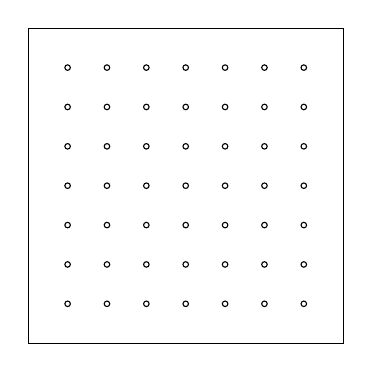
\begin{tikzpicture}
    \draw(0,0) rectangle (4,4);
    \foreach \x in {0.5,1,1.5,2,2.5,3,3.5}
    \foreach \y in {0.5,1,1.5,2,2.5,3,3.5}
    \draw(\x,\y) circle (1pt);
  \end{tikzpicture}
  \caption{A regular grid generated easily with two for loops.}\label{fig:tikz_example}
\end{figure}
\end{ltgexample}

\section{Plots with pgfplots}

The \href{https://ctan.org/pkg/pgfplots}{pgfplots} package plots functions directly in \LaTeX{}, similar to MATLAB or gnuplot.
Some visual examples are available in the package documentation\footnote{\url{http://texdoc.net/pkg/pgfplots}}.

\begin{ltgexample}
\begin{figure}[ht]
  \centering
  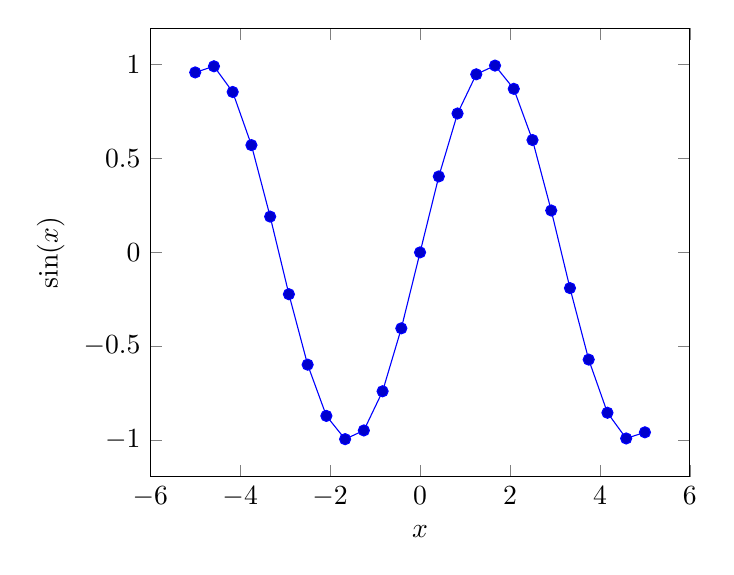
\begin{tikzpicture}
    \begin{axis}[xlabel=$x$, ylabel=$\sin(x)$]
      \addplot {sin(deg(x))};  % Plot the sine function
    \end{axis}
  \end{tikzpicture}
  \caption{Plot of $\sin(x)$ directly inside the figure environment with pgfplots.}
  \label{fig:pgfplots_example}
\end{figure}
\end{ltgexample}

Coordinates can also be given explicitly instead of as a function:
\begin{ltgexample}
\begin{figure}[ht]
  \centering
  \begin{tikzpicture}
    \begin{axis}[xlabel=$x$, ylabel=$y$]
      \addplot coordinates {(0,0) (1,1) (2,4) (3,9)};  % Plot explicit coordinates
    \end{axis}
  \end{tikzpicture}
  \caption{Explicit coordinates plotted with pgfplots.}
  \label{fig:pgfplots_coords}
\end{figure}
\end{ltgexample}

\section{Tables}

\begin{ltgexample}
\begin{table}
  \caption{Simple Table}
  \label{tab:simple}
  \centering
  \begin{tabular}{ll}
    \toprule
    Heading1 & Heading2 \\
    \midrule
    One      & Two      \\
    Thee     & Four     \\
    \bottomrule
  \end{tabular}
\end{table}
\end{ltgexample}

\begin{ltgexample}
% Source: https://tex.stackexchange.com/a/468994/9075
\begin{table}
  \caption{Table with diagonal line}
  \label{tab:diag}
  \begin{center}
    \begin{tabular}{|l|c|c|}
      \hline
      \diagbox[width=10em]{Diag \\Column Head I}{Diag Column\\Head II} & Second & Third \\
      \hline
                                                                       & foo    & bar   \\
      \hline
    \end{tabular}
  \end{center}
\end{table}
\end{ltgexample}


\section{Tables spanning multiple pages}

The \href{https://ctan.org/pkg/longtable}{longtable} package typesets tables that automatically break across page boundaries.
The header (\verb+\endhead+) and footer (\verb+\endfoot+) rows are repeated on every page; once enough rows are added, the table spans several pages on its own.

\begin{ltgexample}
\begin{longtable}{|l|l|l|}
  \caption{A sample long table.}\label{tab:long} \\
  \hline
  \multicolumn{1}{|c|}{\textbf{First column}} & \multicolumn{1}{c|}{\textbf{Second column}} & \multicolumn{1}{c|}{\textbf{Third column}} \\ \hline
  \endfirsthead

  \multicolumn{3}{c}{{\bfseries \tablename\ \thetable{} -- continued from previous page}} \\
  \hline
  \multicolumn{1}{|c|}{\textbf{First column}} & \multicolumn{1}{c|}{\textbf{Second column}} & \multicolumn{1}{c|}{\textbf{Third column}} \\ \hline
  \endhead

  \hline \multicolumn{3}{|r|}{{Continued on next page}} \\ \hline
  \endfoot

  \hline\hline
  \endlastfoot

  A & BC & D \\
  A & BC & D \\
  A & BC & D \\
  A & BC & D \\
  A & BC & D \\
  A & BC & D \\
  A & BC & D \\
  A & BC & D \\
  A & BC & D \\
  A & BC & D \\
  A & BC & D \\
  A & BC & D \\
\end{longtable}
\end{ltgexample}

\section{Source Code}

\begin{ltgexample}
\Zcref{lst:XML} shows source code written in XML.
\Zcref{line:comment} contains a comment.

\begin{lstlisting}[
  language=XML,
  caption={Example XML Listing},
  label={lst:XML}]
<listing name="example">
  <!-- comment --> (* \label{line:comment} *)
  <content>not interesting</content>
</listing>
\end{lstlisting}
\end{ltgexample}

One can also add \verb+float+ as parameter to have the listing floating.
\Zcref{lst:flXML} shows the floating listing.

\begin{ltgexample}
\begin{lstlisting}[
  % one can adjust spacing here if required
  % aboveskip=2.5\baselineskip,
  % belowskip=-.8\baselineskip,
  float,
  language=XML,
  caption={Example XML listing -- placed as floating figure},
  label={lst:flXML}]
<listing name="example">
  Floating
</listing>
\end{lstlisting}
\end{ltgexample}

One can also typeset JSON as shown in \zcref{lst:json}.

\begin{ltgexample}
\begin{lstlisting}[
  float,
  language=json,
  caption={Example JSON listing -- placed as floating figure},
  label={lst:json}]
{
  key: "value"
}
\end{lstlisting}
\end{ltgexample}

Java is also possible as shown in \zcref{lst:java}.

\begin{ltgexample}
\begin{lstlisting}[
  caption={Example Java listing},
  label=lst:java,
  language=Java,
  float]
public class Hello {
    public static void main (String[] args) {
        System.out.println("Hello World!");
    }
}
\end{lstlisting}
\end{ltgexample}

\section{Itemization}

One can list items as follows:

\begin{ltgexample}
\begin{itemize}
  \item Item One
  \item Item Two
\end{itemize}
\end{ltgexample}

With the package paralist, one can create itemizations with lesser spacing:

\begin{ltgexample}
\begin{compactitem}
  \item Item One
  \item Item Two
\end{compactitem}
\end{ltgexample}

One can enumerate items as follows:

\begin{ltgexample}
\begin{enumerate}
  \item Item One
  \item Item Two
\end{enumerate}
\end{ltgexample}

With the package paralist, one can create enumerations with lesser spacing:

\begin{ltgexample}
\begin{compactenum}
  \item Item One
  \item Item Two
\end{compactenum}
\end{ltgexample}

With paralist, one can even have all items typeset after each other and have them clean in the TeX document:

\begin{ltgexample}
\begin{inparaenum}
  \item All these items...
  \item ...appear in one line
  \item This is enabled by the paralist package.
\end{inparaenum}
\end{ltgexample}

\section{Abbreviations}

With \verb+\gls{...}+ you can enter abbreviations, the first time you call it, the long form is used.
When reusing \verb+\gls{..}+ the short form is automatically displayed.
The abbreviation is also automatically inserted in the abbreviation list.
With \verb+\glspl{...}+ the plural form is used.
If you want the short form to appear directly at the first use, you can use \verb+\glsunset{..}+ to mark an abbreviation as already used.
The opposite is achieved with \verb+\glsreset{..}+.

Abbreviations are defined in \verb+\content\ausarbeitung.tex+ by means of \verb+\newacronym{...}{...}{...}+.

More information at: \url{https://ctan.org/pkg/bib2gls}.

\begin{ltgexample}
At the first pass, the \gls{er} was 5.
At the second pass was \gls{er} 3.
The plural form can be seen here: \glspl{er}.
To demonstrate what the list of abbreviations looks like for longer description texts, \glspl{rdbms} must be mentioned here.

\gls{dante} is a local \TeX\ user group.
The German-speaking local \TeX\ user group is \gls{dante}.
A \gls{gp} is a medical doctor.
I went to my surgery to see the \gls{gp}.
\end{ltgexample}

\todo{Include difference between acronym and abbreviation - \url{https://tex.stackexchange.com/a/154566/9075}}

\section{Other Features}

\begin{ltgexample}
The words \enquote{workflow} and \enquote{dwarflike} can be copied from the PDF and pasted to a text file.
\end{ltgexample}

\begin{ltgexample}
The symbol for powerset is now correct: $\powerset$ and not a Weierstrass p ($\wp$).

$\powerset({1,2,3})$
\end{ltgexample}

\begin{ltgexample}
Brackets work as designed:
<test>
One can also input backticks in verbatim text: \verb|`test`|.
\end{ltgexample}

Acronyms can be typeset in running text with \verb+\initialism+, which sets them as small caps that blend into the surrounding lowercase text. It is the lightweight alternative to the full acronym and glossary management (\verb+\gls+, with an automatic list of abbreviations) provided by the thesis variants: \verb+\initialism+ only typesets the acronym and does not add it to any list. The macro and a few ready-made acronyms (\verb+\OMG+, \verb+\BPEL+, \verb+\BPMN+, \verb+\UML+) are defined in \texttt{commands.tex}, where you can add your own.

\begin{ltgexample}
The \UML is maintained by the \OMG; related standards include \BPEL and \BPMN.
Any acronym can be set inline with \initialism{REST} or \initialism{HTTP}.
\end{ltgexample}


\section{Zref-vario examples}
\label{sec:ex:vref}

zref-vario demonstration: zvref[S] at beginning of sentence, zvref in all other cases.

\begin{ltgexample}
\zvref[S]{fig:ex:cref} shows a simple fact, although \zvref{fig:ex:cref} could also show something else.

\zvref[S]{tab:ex:cref} shows a simple fact, although \zvref{tab:ex:cref} could also show something else.

\zvref[S]{sec:ex:cref} shows a simple fact, although \zvref{sec:ex:cref} could also show something else.
\end{ltgexample}

\section{Citations}

When referencing something from the bibliography file, it will automatically appear in the references section.
If a reference is not cited, it is not appearing there.

\begin{ltgexample}
Standard case: Citing indirectly citing something~\cite{mwe}.
In case one wants to name the author: \textcite{mwe} shows a minimal \LaTeX{} example.
\end{ltgexample}

Note that \texttt{\textbackslash textcite\{mwe\}} prints both the author and the reference to the bibliography entry.

Remember that you have to call \texttt{biber main-english} to generate the bibliography data for \texttt{lualatex}.
You will need to run \texttt{lualatex} twice so that the page numbers are up to date.


In the bibliography, use \texttt{\textbackslash textsuperscript} for \enquote{st}, \enquote{nd}, \ldots:
E.g., \enquote{The 2\textsuperscript{nd} conference on examples}.
When you use \href{https://www.jabref.org}{JabRef}, you can use the clean up command to achieve that.
See \url{https://help.jabref.org/en/CleanupEntries} for an overview of the cleanup functionality.

\section{Miscellaneous Examples}
\label{ssec:example}

Reference test: \Zcref{ssec:example}, \zcref{fig:Abbildung} and \zcref{alg:example}.

\begin{ltgexample}
Checkmark: \dingcheck.
Crossmark: \dingcross.
\end{ltgexample}

\begin{figure}
  \missingfigure{}
  \caption{Figure}
  \label{fig:Abbildung}
\end{figure}

\begin{landscape}
  \begin{figure}
    \missingfigure{}
    \caption{Rotated figure}
    \label{fig:AbbildungGedreht}
  \end{figure}
\end{landscape}

\subsection{Algorithms}

\begin{algorithm}
  \caption{$algo$}
  \label{alg:example}
  \begin{algorithmic}[1]
    \State $a \gets 0$
    \State State 2\label{alg1:state2}
  \end{algorithmic}
\end{algorithm}

\begin{algorithm}
  \caption{Algorithm 2}
  \label{alg:example2}
  \begin{algorithmic}[1]
    \State $a \gets 0$
    \State State 2\label{alg2:state2}
  \end{algorithmic}
\end{algorithm}

\Zcref{alg:example} has already shown an algorithm.
Test of line referencing: line~\ref{alg1:state2} (\zcref{alg:example}) and line~\ref{alg2:state2} (\zcref{alg:example2}).

\subsection{Definitions}
\begin{definition}[Title]
  \label{def:def1}
  Definition Text
\end{definition}

\Zcref{def:def1} shows \ldots

\subsection{Enumerations}

\begin{enumerate}[label=\alph*)]
  \item a
  \item b
  \item c
  \item d
\end{enumerate}

Equivalent to paralist's inparaenum:
\begin{enumerate*}[label=\alph*)]
  \item a
  \item b
  \item c
  \item d
\end{enumerate*}

\begin{description}
  \item[first] First
  \item[second] Second
  \item[third] Third
\end{description}

\begin{description}
  \item[\texttt{first}] First
  \item[\texttt{second}] Second
  \item[\texttt{third}] Third
\end{description}

%works only if package enumitem is loaded
\begin{description}[font=\ttfamily]
  \item[first] First
  \item[second] Second
  \item[third] Third
\end{description}

\begin{description}[style=unboxed]
  \item[first label with a long description text breaking over one line. Enabled by enumitem package] First
  \item[second] Second
  \item[third] Third
\end{description}

\begin{Description}
  \item[first label with a long description text breaking over one line. Defined in template.tex] First
  \item[second] Second
  \item[third] Third
\end{Description}

\begin{itemize}
  \item First
  \item Second
  \item Third
\end{itemize}

The optional parameter changes the marker that is prepended.
See \url{http://www.weinelt.de/latex/item.html}.
\begin{itemize}
  \item[A] First
  \item[B] Second
  \item[C] Third
\end{itemize}

Incorrect use of the optional parameter as follows:
\begin{itemize}
  \item[first] First
  \item[second] Second
  \item[third] Third
\end{itemize}
Note that, when \texttt{enumitem} is loaded, this behaves differently than with \texttt{paralist}.

\subsection{fquote}

\begin{fquote}[T.\ Scientist]
  The program will be finished by next Friday.
\end{fquote}

\begin{gfquote}{T.\ Scientist}
  The program will be finished by next Friday.
\end{gfquote}
